\documentclass[tikz,border=5pt]{standalone}
\usepackage[utf8]{inputenc}
\usepackage[T1]{fontenc}
\usepackage{amsmath,amssymb}
\usepackage{lmodern}
\usetikzlibrary{arrows.meta}

\definecolor{ink}{HTML}{1d1d1f}
\definecolor{sub}{HTML}{515154}
\definecolor{muted}{HTML}{6e6e73}
\definecolor{border}{HTML}{d2d2d7}
\definecolor{mist}{HTML}{f5f5f7}
\definecolor{amber}{HTML}{c76008}
\definecolor{amberbright}{HTML}{ff9f0a}
\definecolor{amberfill}{HTML}{fff3e0}
\definecolor{green}{HTML}{1a7f37}
\definecolor{greenbright}{HTML}{30d158}
\definecolor{greenfill}{HTML}{dcf7e3}
\definecolor{red}{HTML}{d70015}
\definecolor{redbright}{HTML}{ff453a}

\begin{document}
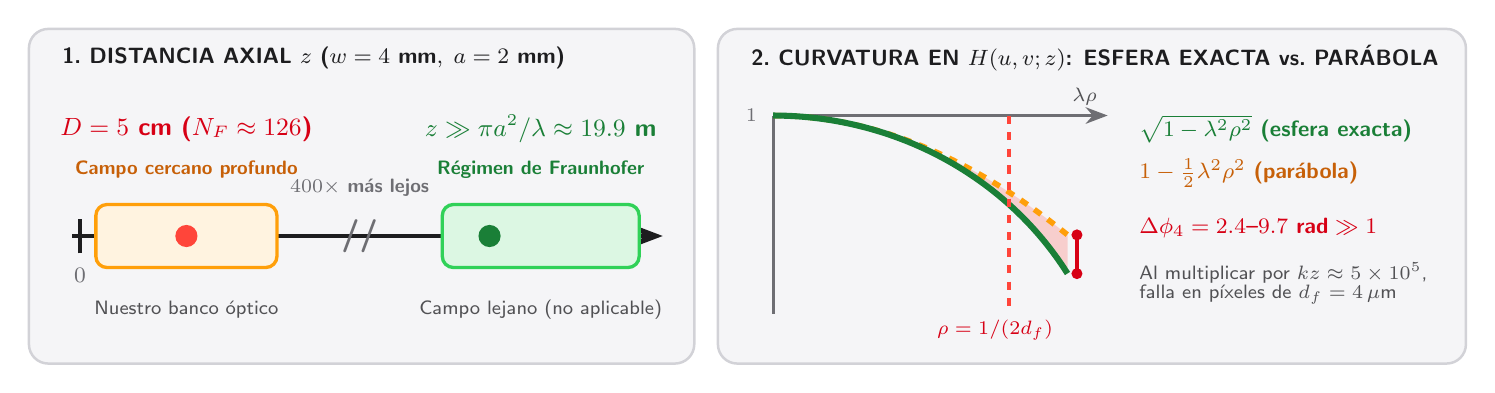
\begin{tikzpicture}[font=\sffamily,>=Stealth]

% ===================== PANEL 1: REGLA AXIAL z =====================
\draw[border,fill=mist,rounded corners=7pt,line width=0.9pt] (0,0) rectangle (8.45,4.25);
\node[anchor=west,font=\sffamily\footnotesize\bfseries,text=ink] at (0.30,3.88)
  {1.\ DISTANCIA AXIAL $z$ ($w = 4\text{ mm},\; a = 2\text{ mm}$)};

% Eje z
\draw[->,ink,line width=1.6pt] (0.55,1.62) -- (8.05,1.62);
\draw[ink,line width=1.6pt] (0.65,1.40) -- (0.65,1.84);
\node[font=\sffamily\footnotesize\bfseries,text=muted] at (0.65,1.12) {$0$};

% Nuestro montaje D = 5 cm
\draw[amberbright,fill=amberfill,rounded corners=4pt,line width=1.2pt] (0.85,1.22) rectangle (3.15,2.02);
\fill[redbright] (2.00,1.62) circle (4pt);
\node[font=\sffamily\small\bfseries,text=red] at (2.00,2.98) {$D = 5\text{ cm}$ ($N_F \approx 126$)};
\node[font=\sffamily\scriptsize\bfseries,text=amber] at (2.00,2.46) {Campo cercano profundo};
\node[font=\sffamily\scriptsize,text=sub] at (2.00,0.68) {Nuestro banco óptico};

% Salto 400x (más centrado en el hueco libre 3.15..5.25)
\node[font=\sffamily\large\bfseries,text=muted] at (4.20,1.62) {//};
\node[font=\sffamily\scriptsize\bfseries,text=muted] at (4.20,2.24) {$400\times$ más lejos};

% Fraunhofer z >> 19.9 m
\draw[greenbright,fill=greenfill,rounded corners=4pt,line width=1.2pt] (5.25,1.22) rectangle (7.75,2.02);
\fill[green] (5.85,1.62) circle (4pt);
\node[font=\sffamily\small\bfseries,text=green] at (6.50,2.98) {$z \gg \pi a^2 / \lambda \approx 19.9\text{ m}$};
\node[font=\sffamily\scriptsize\bfseries,text=green] at (6.50,2.46) {Régimen de Fraunhofer};
\node[font=\sffamily\scriptsize,text=sub] at (6.50,0.68) {Campo lejano (no aplicable)};

% ===================== PANEL 2: ESFERA vs PARÁBOLA DE FRESNEL =====================
\draw[border,fill=mist,rounded corners=7pt,line width=0.9pt] (8.75,0) rectangle (18.25,4.25);
\node[anchor=west,font=\sffamily\footnotesize\bfseries,text=ink] at (9.05,3.88)
  {2.\ CURVATURA EN $H(u,v;z)$: ESFERA EXACTA vs.\ PARÁBOLA};

% Sistema de coordenadas interno para plotear x = lambda * rho in [0, 0.86]
\begin{scope}[shift={(9.45,3.15)}]
  % Ejes de referencia
  \draw[->,muted,line width=1.1pt] (0,0) -- (4.25,0) node[above left,font=\sffamily\scriptsize\bfseries,text=sub]{$\lambda\rho$};
  \draw[muted,line width=1.1pt] (0,0) -- (0,-2.52);
  \node[anchor=east,font=\sffamily\scriptsize\bfseries,text=muted] at (-0.08,0) {$1$};

  % Área de error entre parábola y esfera: 1 - 0.5 x^2  vs  sqrt(1 - x^2)
  \fill[redbright,opacity=0.22]
    plot[domain=0:0.86,samples=50] ({4.35*\x}, {4.1*(-0.5*\x*\x)}) --
    plot[domain=0.86:0,samples=50] ({4.35*\x}, {4.1*(sqrt(1-\x*\x)-1)}) -- cycle;

  % Parábola de Fresnel: 1 - 0.5 x^2
  \draw[amberbright,dashed,line width=2.0pt]
    plot[domain=0:0.86,samples=60] ({4.35*\x}, {4.1*(-0.5*\x*\x)});

  % Esfera exacta: sqrt(1 - x^2)
  \draw[green,line width=2.2pt]
    plot[domain=0:0.86,samples=60] ({4.35*\x}, {4.1*(sqrt(1-\x*\x)-1)});

  % Marcador de Nyquist
  \draw[redbright,dashed,line width=1.3pt] (3.00,0) -- (3.00,-2.48);
  \node[font=\sffamily\scriptsize\bfseries,text=red] at (2.82,-2.72) {$\rho = 1/(2d_f)$};

  % Segmento limpio de brecha sin flechas encimadas
  \draw[red,line width=1.6pt] (3.86,{4.1*(-0.5*0.86*0.86)}) -- (3.86,{4.1*(sqrt(1-0.86*0.86)-1)});
  \fill[red] (3.86,{4.1*(-0.5*0.86*0.86)}) circle (2pt);
  \fill[red] (3.86,{4.1*(sqrt(1-0.86*0.86)-1)}) circle (2pt);
\end{scope}

% Leyenda del Panel 2 a la derecha (bien separada de la gráfica)
\node[anchor=west,font=\sffamily\footnotesize\bfseries,text=green] at (13.98,2.98)
  {$\sqrt{1 - \lambda^2\rho^2}$ (esfera exacta)};
\node[anchor=west,font=\sffamily\footnotesize\bfseries,text=amber] at (13.98,2.42)
  {$1 - \frac{1}{2}\lambda^2\rho^2$ (parábola)};
\node[anchor=west,font=\sffamily\footnotesize\bfseries,text=red] at (13.98,1.72)
  {$\Delta\phi_4 = 2.4\text{--}9.7\text{ rad} \gg 1$};
\node[anchor=west,font=\sffamily\scriptsize,text=sub,align=left] at (13.98,1.02)
  {Al multiplicar por $kz \approx 5\times 10^5$,\\[-1pt]falla en píxeles de $d_f = 4\,\mu\text{m}$};

\end{tikzpicture}
\end{document}
